% !TEX root = Projektstudie.tex
% Mathematik


\section{Mathematische Modellierung}
\label{sec:Mathematische Modellierung}
\begin{figure}
    \centering
    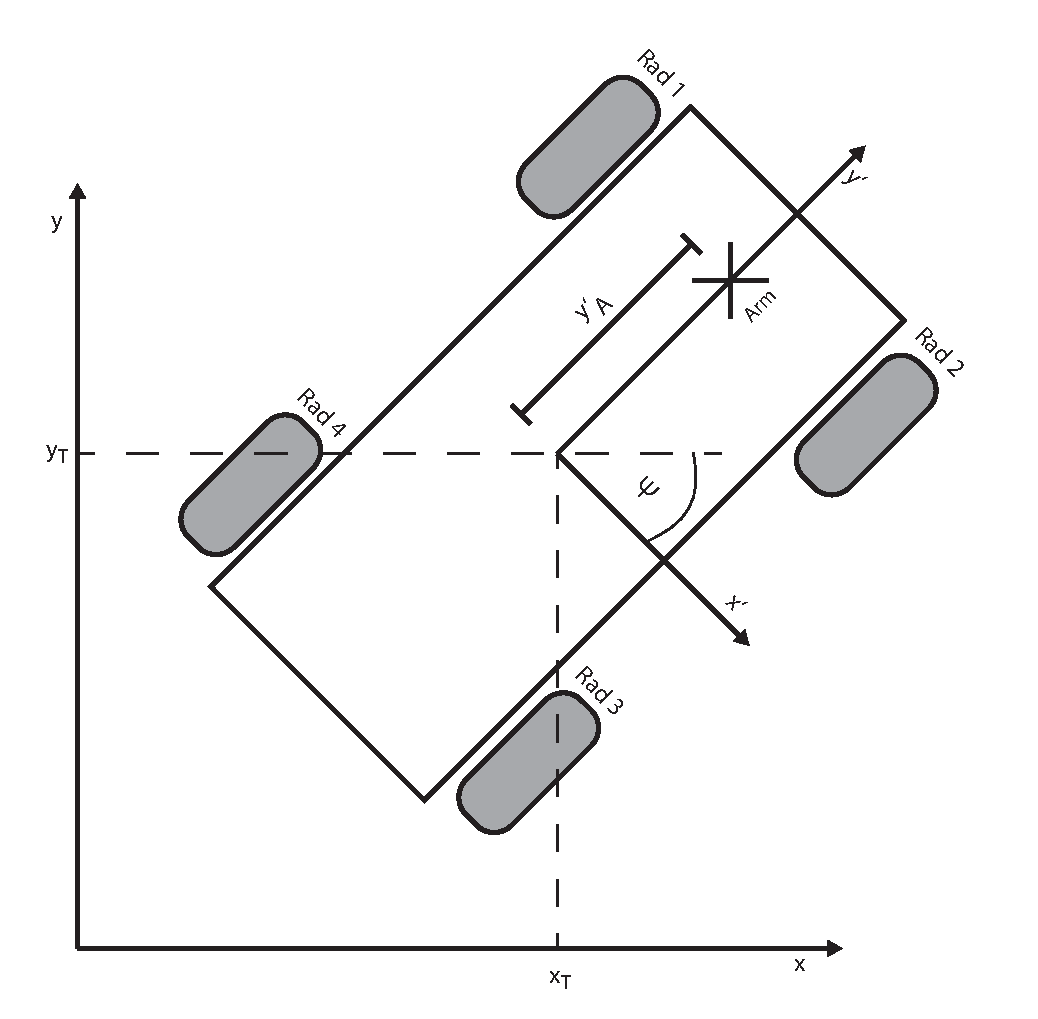
\includegraphics[width=.8\textwidth]{Abbildungen/Koordinaten}
    \caption{Einführung der verwendeten Koordinatensysteme, der Position des Arms sowie der Radnummerierung.}
\end{figure}
Dieses Kapitel beschreibt die Mathematik hinter der Kinematik und Dynamik des Mecanum-Roboters.
Jede Bewegung setzt sich aus einer translatorischen und einer rotatorischen Teilbewegung zusammen.

\subsection{Translation}
\label{sec:Translation}
Um eine translatorische Bewegung auszuführen, werden die Räder paarweise (1+3, 2+4) mit gleicher Drehrichtung und Drehgeschwindigkeit angetrieben.
Die resultierende Gesamtkraft bestimmt die Richtung der Fahrt.
Die folgenden Rechnungen behandeln die Ermittlung der einzelnen Soll-Radgeschwindigkeiten aus einem vorgegebenen Geschwindigkeitsvektor.

\begin{figure}[H]
    \centering
    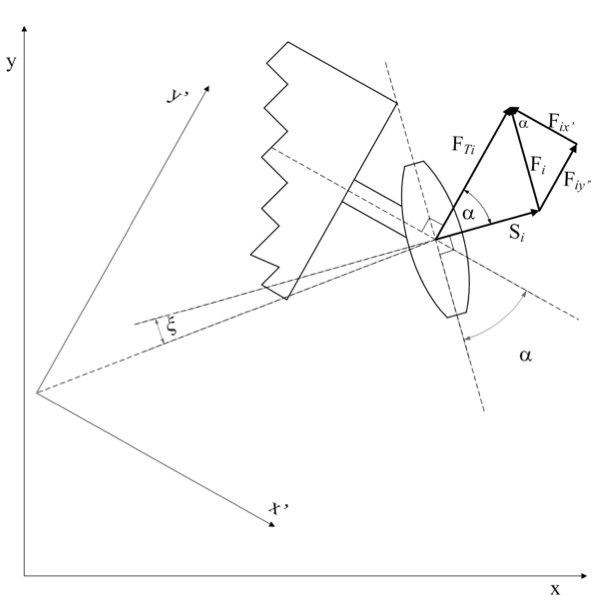
\includegraphics[width=.6\textwidth]{Abbildungen/Kraefte-am-Rad}
    \caption{Kräftegleichgewicht an einem Mecanum-Rad.}
\end{figure}

Die Leistung einer vektoriellen Kraft berechnet sich nach : 
$$ P_F = F_T \cdot v_F $$

Wirken Kraft und Geschwindigkeit entlang einer Koordinatenachse, haben beide Vektoren die gleiche Komponente ungleich null und ihr Skalarprodukt kann vereinfacht als Produkt der skalaren Größen betrachtet werden.

Die Kraftvektor in $x$- und $y$-Richtung setzt sich zusammen als die Summe der einzelnen $x$- und $y$-Vektoren der vier Räder:
\begin{align*}
    \sum_{i=1}^4 F_{ix} &= \sum_{i=1}^4 F_i \cos \alpha \\
    &= \sum_{i=1}^4 (-1)^i SIG \cdot K_i F_{Ti} \sin \alpha \cos \alpha \\
    &= \sum_{i=1}^4 (-1)^i SIG \cdot \frac{1}{2} K_i F_{Ti}
\end{align*}
\begin{align*}
    \sum_{i=1}^4 F_{iy} &= \sum_{i=1}^4 F_i \sin \alpha \\
    &= \sum_{i=1}^4 SIG \cdot K_i F_{Ti} \sin^2 \alpha \\
    &= \sum_{i=1}^4 SIG \cdot \frac{1}{2} K_i F_{Ti}
\end{align*}

SIG sei die Vorzeichenkonventionen für die Drehrichtung der Räder.
Diese wird in der Steuerung direkt implementiert und wird daher bei den folgenden Rechnungen nicht weiter betrachtet.

Der Winkel $ \alpha $ beschreibt den Winkel, in dem die Rollen auf dem Mecanum-Rad angebracht sind.
In den meisten Fällen gilt $\alpha = 45^\circ$.

Für eine translatorische Bewegung müssen die Radpaare mit gleicher Geschwindigkeit drehen.
Entsprechend müssen ihre Kraftvektoren $F_{T1, 3} / F_{T2, 4}$ gleich groß sein.
Durch Auflösen der Summenzeichen erhält man ein Gleichungssystem:
\begin{align*}
    F_x &= - K_i F_{T1, 3} + K_i F_{T2, 4} \\
    F_y &= K_i F_{T1, 3}   + K_i F_{T2, 4}
\end{align*}

Nach dem Umstellen erhält man $F_{T1, 3}$ und $F_{T2, 4}$ und kann somit auch direkt die Geschwindigkeiten berechnen:
\begin{align*}
    F_{T1, 3} &= \frac{F_y + F_x}{K_i} &\Rightarrow v_{T1, 3} &= \frac{v_y + v_x}{K_i} \\
    F_{T2, 4} &= \frac{F_y - F_x}{K_i} &\Rightarrow v_{T2, 4} &= \frac{v_y - v_x}{K_i} \\
\end{align*}

Der Faktor $K_i$ setzt sich aus unterschiedlichen Einzelfaktoren zusammen, welche die durch das Motormoment erzeugten treibenden Kräfte beeinflussen. $K_i$ wird für den Boden der Werkstatt empirisch ermittelt. Die Beschreibung der durchgeführten Versuchsreihe folgt in Kapitel~\ref{sec:versuche-k-faktor}.


\subsection{Rotation}
\label{sec:Rotation}
Die Rotation des Mecanum-Roboters um sein Zentrum müssen alle Räder mit gleicher Geschwindigkeit drehen, lediglich die Richtung unterscheidet sich.
Für eine Drehung im Uhrzeigersinn drehen beispielsweise Rad 1 und 2 rückwärts, Rad 3 und 4 vorwärts. Allgemein gilt:
\begin{align*}
    v_{ref} &= K_i \cdot r \cdot \omega \\
    v_1 = v_4 &= - v_{ref} \\
    v_2 = v_3 &= + v_{ref}
\end{align*}

\subsection{Versuchsreihe: Bestimmung $K_i$}
\label{sec:versuche-k-faktor}

Der Faktor $K_i$ hat einen großen Einfluss auf die Bewegung des Mecanum-Roboters. Er setzt sich aus unterschiedlichen Einzelfaktoren zusammen, welche die durch das Motormoment erzeugten treibenden Kräfte beeinflussen. Zu den Einflussfaktoren zählen unter anderem die verschiedenen Reibungsfaktoren und die Flächenträgheitsmomente. Da eine Bestimmung der einzelnen Faktoren sehr aufwendig wäre und die Varianzen der Fehleranteile  bei der Multiplikation zu $K_i$ ebenfalls multipliziert werden müssen, wird $K_i$ direkt empirisch ermittelt. 

Bei diversen Probefahrten wird ein sehr großer Einfluss des Untergrunds festgestellt. Die Bestimmung für  $K_i$  erfolgt daher explizit für den Boden in der Werkstatt. Um den Einfluss von Staub und anderen äußeren Faktoren gering zu halten, wird die Versuchsreihe unter folgenden definierten Bedingungen durchgeführt:

\begin{itemize}
\item gefegt
\item trocken 
\item ölfrei
\end {itemize}

Unebenheiten, welche aufgrund der Funktionsweise der Mecanum-Räder einen ebenfalls einen großen Einfluss haben, können aus Praktikabilitätsgründen nicht berücksichtigt werden. Für die Versuchsreihe wird daher eine möglichst ebene Versuchsstrecke ausgewählt. Je länger die Strecke ist, desto größer ist die Gefahr von Unebenheiten. Bei einer sehr kurzen Strecke und entsprechend kurzen Messzeiten ist die Reproduzierbarkeit nicht gewährleistet. 

Als günstiger Kompromiss wird eine fünf Meter lange Versuchsstrecke auf dem Flur ausgewählt. Um zusätzlich eine mögliche  Richtungsabhängigkeit des Faktors zu untersuchen werden acht Fahrrichtungen untersucht. Die Fahrzeit wird jeweils von zwei Stoppuhren erfasst. 








